% !TEX program = lualatex
\documentclass[10pt,a4paper]{article}
\usepackage{luatexja-fontspec}
\usepackage{luatexja}
% 明朝体：Noto Serif CJK JP、ゴシック体：Noto Sans CJK JP
\setmainjfont[BoldFont=Noto Serif CJK JP Bold]{Noto Serif CJK JP}
\setsansjfont[BoldFont=Noto Sans CJK JP Bold]{Noto Sans CJK JP}
\usepackage{amsmath,amssymb}
\usepackage{booktabs}
\usepackage{graphicx}
\usepackage{xcolor}
\usepackage{hyperref}
\usepackage[margin=2.2cm]{geometry}
\usepackage{caption}
\usepackage{subcaption}
\usepackage{parskip}
\usepackage{enumitem}
\usepackage{fancyhdr}
\usepackage{titlesec}
\usepackage{tcolorbox}
\usepackage{float}
\usepackage{microtype}

\hypersetup{colorlinks=true, linkcolor=blue!70!black, citecolor=blue!70!black, urlcolor=blue!70!black}
\titleformat{\section}{\large\bfseries\color{blue!60!black}}{}{0em}{}[\titlerule]
\titleformat{\subsection}{\normalsize\bfseries\color{blue!40!black}}{}{0em}{}
\setlength{\parskip}{4pt}
\pagestyle{fancy}
\fancyhf{}
\rhead{\small NIFE/IKM 内部レポート}
\lhead{\small Dieckow Analysis --- 日本語版}
\cfoot{\small \thepage}

\tcbuselibrary{skins}
\newtcolorbox{keybox}[1][]{colback=blue!5!white, colframe=blue!50!black,
  fonttitle=\bfseries, title=#1, left=4pt, right=4pt, top=3pt, bottom=3pt}
\newtcolorbox{limitbox}[1][]{colback=red!5!white, colframe=red!40!black,
  fonttitle=\bfseries, title=#1, left=4pt, right=4pt, top=3pt, bottom=3pt}

\newcommand{\bphi}{\boldsymbol{\phi}}
\newcommand{\bA}{\mathbf{A}}
\newcommand{\bb}{\mathbf{b}}

\title{%
  \textbf{代謝プライア付き Replicator 力学による\\
  経口マイクロバイオーム組成の予測\\
  --- LOO 交差検証による評価 ---}\\[6pt]
  \large \textit{NIFE/IKM 内部レポート --- Nishioka \& Szafra\'{n}ski, \today}
}
\author{}
\date{}

\begin{document}
\maketitle\thispagestyle{fancy}
\vspace{-1em}

% ── 要旨 ─────────────────────────────────────────────────────────────
\begin{abstract}
\noindent
フラックスバランス解析 (FBA) から導かれる代謝ネットワーク制約が、
経口マイクロバイオームのコミュニティ動態の予測精度を改善するかを検証した。
eHOMD 実験代謝フロー (L1) と AGORA2 pFBA クロスフィーディング予測 (L2+L3)
による 3 層サインプライアを組み込んだ Hamilton Replicator ODE を、
Dieckow et~al.~(2024) のう蝕回復中 10 患者の 16S rRNA アンプリコンデータ
（週 1 回 $\times$ 3 週、10 クラスレベルギルド）にフィットした。
Leave-one-patient-out (LOO) 交差検証の結果：
\textbf{LOO-RMSE $= 0.0504 \pm 0.021$}（AGORA W$=1.0$、非拘束 gLV 比 $-14\%$）、
\textbf{LOO Bray-Curtis $= 0.147$}（持続性ヌルモデル比 $-48\%$）。
重み $w=1.0$ で離散的相転移が生じ、符号一致率 70/70（100\%）を達成。
独立したインプラント周囲炎データセット 127 例での外部検証では、
推定した相互作用行列がコミュニティ Dysbiosis の重症度を正しく順序付けた
（Kruskal-Wallis $p < 0.0001$、Spearman $\rho = 0.37$）。
主な限界は $N=10$（検出力不足、$p=0.08$）、対称 $\bA$ 制約、
およびう蝕文脈に偏ったプライアである。
\end{abstract}

\tableofcontents\bigskip

% ── 1. 背景と動機 ────────────────────────────────────────────────────
\section{背景と動機}

経口マイクロバイオームは、歯周病・う蝕の病態基盤となる
空間構造を持つ合成栄養コミュニティである。
縦断的 16S rRNA データは時間断面を提供するが、
一般化 Lotka-Volterra (gLV) 相互作用行列 $\bA$（パラメータ数 $K^2 \sim 100$）は、
$N=10$ 患者 $\times$ $T=3$ 時点のデータから決定するには厳しく劣決定である。

通常の $L_2/L_1$ 正則化は全相互作用を等価に扱うが、
代謝的根拠に基づく代替手法として、
「ギルド $j$ がギルド $i$ の消費する代謝産物を産生する」ならば
大きさに関わらず $A_{ij}>0$ と符号を制約する方法がある。

Szafra\'{n}ski et~al.~(2025) は、
eHOMD（Expanded Human Oral Microbiome Database）と AGORA2 ゲノムスケール代謝モデルから、
10 の経口ギルドレベル分類群に対する実験的・計算的代謝フローを提供している。

本研究はこの 3 層プライアを、Hamilton Replicator（対称 $\bA$、
拡張 Hamilton 原理から導かれる自由エネルギーの 2 次変分として自然に対称性が要請される）
と JAX 自動微分最適化と組み合わせ、
LOO 交差検証による真の汎化性能を評価する。

% ── 2. 手法 ──────────────────────────────────────────────────────────
\section{手法}

\subsection{データセット}

Dieckow et~al.~(2024)：チタン製インプラントアバットメント上の縁下プラーク、
10 患者（A--H, K, L）、週 1 回 $\times$ 3 週（W1, W2, W3）。
ASV を 10 クラスレベルギルドに集約（表~\ref{tab:guilds}）。

\begin{table}[H]
\centering\small
\caption{10 ギルド定義（SILVA 138.1 クラスレベル）。}
\label{tab:guilds}
\begin{tabular}{lll}
\toprule
Index & ギルド & SILVA クラス \\
\midrule
0 & Actinobacteria      & Actinomycetia \\
1 & Bacilli             & Bacilli \\
2 & Bacteroidia         & Bacteroidia \\
3 & Betaproteobacteria  & Betaproteobacteria \\
4 & Clostridia          & Clostridia, Erysipelotrichia \\
5 & Coriobacteriia      & Coriobacteriia \\
6 & Fusobacteriia       & Fusobacteriia \\
7 & Gammaproteobacteria & Gammaproteobacteria \\
8 & Negativicutes       & Negativicutes, Selenomonadales \\
9 & Other               & その他全て \\
\bottomrule
\end{tabular}
\end{table}

コミュニティ型（CT）：CT1（早期共生優位：Actinobacteria, Bacilli 主体、5 名）vs
CT2（Fusobacteriia, Bacteroidia 優位、5 名）をガウス混合モデルで同定。

\subsection{Hamilton Replicator モデル}

単体上の組成力学を記述する Hamilton Replicator ODE：
\begin{equation}
  \dot\phi_i = \phi_i\bigl(f_i(\bphi) - \bar f(\bphi)\bigr),
  \qquad f_i = b_i + \textstyle\sum_j A_{ij}\phi_j,
  \qquad \bar f = \textstyle\sum_k \phi_k f_k.
\end{equation}
$\phi_i \geq 0$、$\sum_i \phi_i = 1$（平均適応度引算により自動的に維持）。
対称 $A_{ij}=A_{ji}$（Hamilton 原理の自由エネルギー 2 次形式から必然）、
$A_{ii}<0$（自己制限）。JAX-JIT コンパイル済み RK45 積分（$dt=10^{-4}$）。

患者固有の $b_i^{(p)}$ が個体差（免疫状態・抗生剤歴・初期定着歴）を吸収し、
共有 $\bA$ がギルド間の生態学を表す。

\subsection{3 層代謝サインプライア}

\begin{description}[noitemsep]
  \item[L1 --- eHOMD/Szafra\'{n}ski：] 実験的に確認された PRODUCES/USES 関係（34 ペア、$w=2.0$）。
  \item[L2 --- AGORA2 pFBA：] 各ギルドの代表ゲノムスケール代謝モデルに対する
        parsimonious FBA（口腔液標準培地）。1 ペア追加（計 35 ペア）。
  \item[L3 --- AGORA 重みスイープ：] $w_\text{L3} \in \{0.5, 1.0, 1.5, 2.0\}$。
\end{description}

\textbf{ヒンジ 2 乗ペナルティ}（符号違反に 2 次ペナルティ、正符号は 0）：
\begin{equation}
  \mathcal{P}(\bA;\mathbf{F}) = \sum_{(i,j):\,F_{ij}\neq 0}
    \frac{|F_{ij}|}{2\sigma^2}
    \Bigl[\max\!\bigl(0,-\operatorname{sgn}(F_{ij})\cdot A_{ij}\bigr)\Bigr]^2,
  \qquad \sigma = 0.15.
\end{equation}

\textbf{損失関数：}
$\mathcal{L} = \text{RMSE}(\hat\bphi,\bphi) + \mathcal{P}(\bA;\mathbf{F}) + \lambda\|\bA\|_F^2$、
$\lambda=10^{-4}$。L-BFGS-B + JAX 自動微分、最大 5000 反復。

\subsection{Leave-One-Patient-Out 交差検証}

各患者 $p$ をホールドアウト：
(1) $N-1$ 名で $\bA$ と $\{\bb^{(q)}\}_{q\neq p}$ を最適化；
(2) $\bA$ を固定し W1 データのみで $\hat\bb^{(p)}$ を再最適化；
(3) W2, W3 を予測；
(4) RMSE と Bray-Curtis 非類似度 (BC) を評価。

% ── 3. 結果 ──────────────────────────────────────────────────────────
\section{結果}

\subsection{LOO 交差検証の性能}

\begin{table}[H]
\centering\small
\caption{LOO 交差検証まとめ（太字が最良値）。}
\label{tab:loo}
\begin{tabular}{llcccc}
\toprule
モデル & プライア & SA (\%) & LOO-RMSE & Std & LOO-BC \\
\midrule
gLV free（非対称）               & なし       & ---    & 0.0588 & ---   & 0.154 \\
Hamilton（プライアなし）          & なし       & ---    & 0.0595 & 0.024 & ---   \\
Hamilton L1+L2                   & L1+L2      & 94     & 0.0516 & 0.021 & 0.155 \\
\textbf{Hamilton AGORA W1.0}     & L1+L2+L3   & \textbf{100} & \textbf{0.0504} & \textbf{0.021} & \textbf{0.147} \\
Hamilton AGORA W2.0              & L1+L2+L3   & 100    & 0.0505 & ---   & ---   \\
\midrule
持続性ヌル                       & ---        & ---    & ---    & ---   & 0.281 \\
全体平均ヌル                     & ---        & ---    & ---    & ---   & 0.254 \\
\bottomrule
\end{tabular}
\end{table}

\begin{keybox}[数値まとめ]
\begin{itemize}[noitemsep]
  \item LOO-RMSE：\textbf{0.0504}（AGORA W1.0）vs 0.0588（gLV free）$\to$ $\mathbf{-14.3\%}$
  \item LOO-BC：\textbf{0.147} vs 0.281（持続性ヌル）$\to$ $\mathbf{-47.7\%}$
  \item 符号一致率：$w=1.0$ で \textbf{70/70（100\%）}
  \item 10 患者中 7 名が AGORA プライアで改善、患者 L のみ悪化
  \item 対応 $t$ 検定（AGORA vs L1+L2、$N=10$）：$p=0.08$（有意水準直前）
\end{itemize}
\end{keybox}

\begin{figure}[H]
\centering
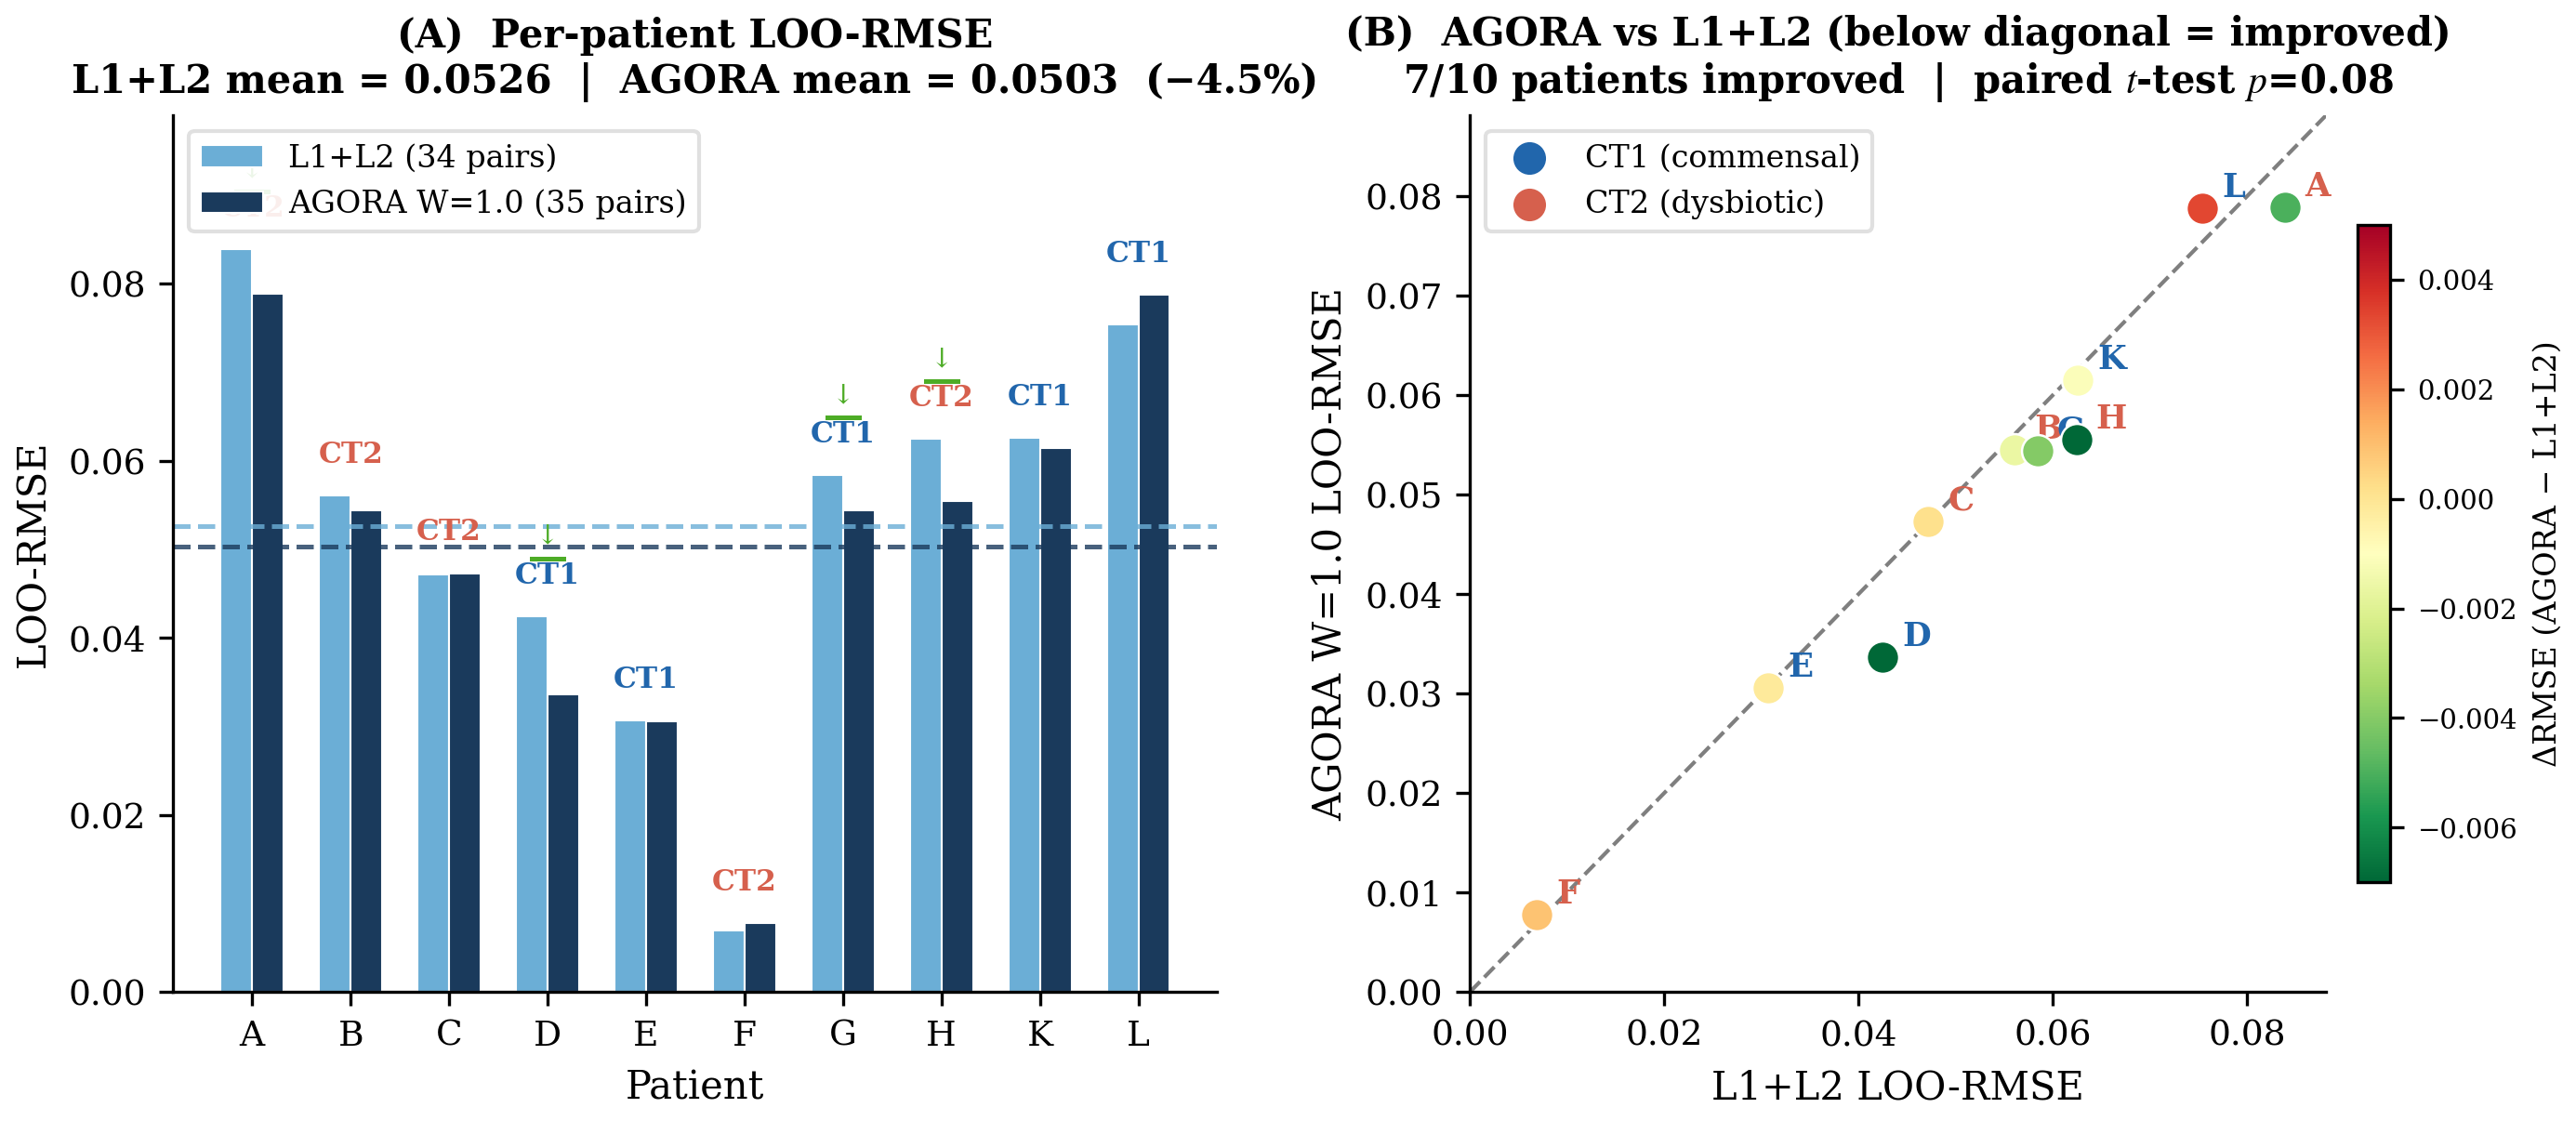
\includegraphics[width=0.88\linewidth]{figures/fig2_loo_comparison.png}
\caption{患者ごとの LOO-RMSE（L1+L2：灰、AGORA W1.0：青）。
10 患者中 7 名で改善。水平破線は gLV free ベースライン。}
\end{figure}

\subsection{相互作用行列と生態学的レジーム}

\begin{figure}[H]
\centering
\begin{subfigure}[b]{0.48\textwidth}
  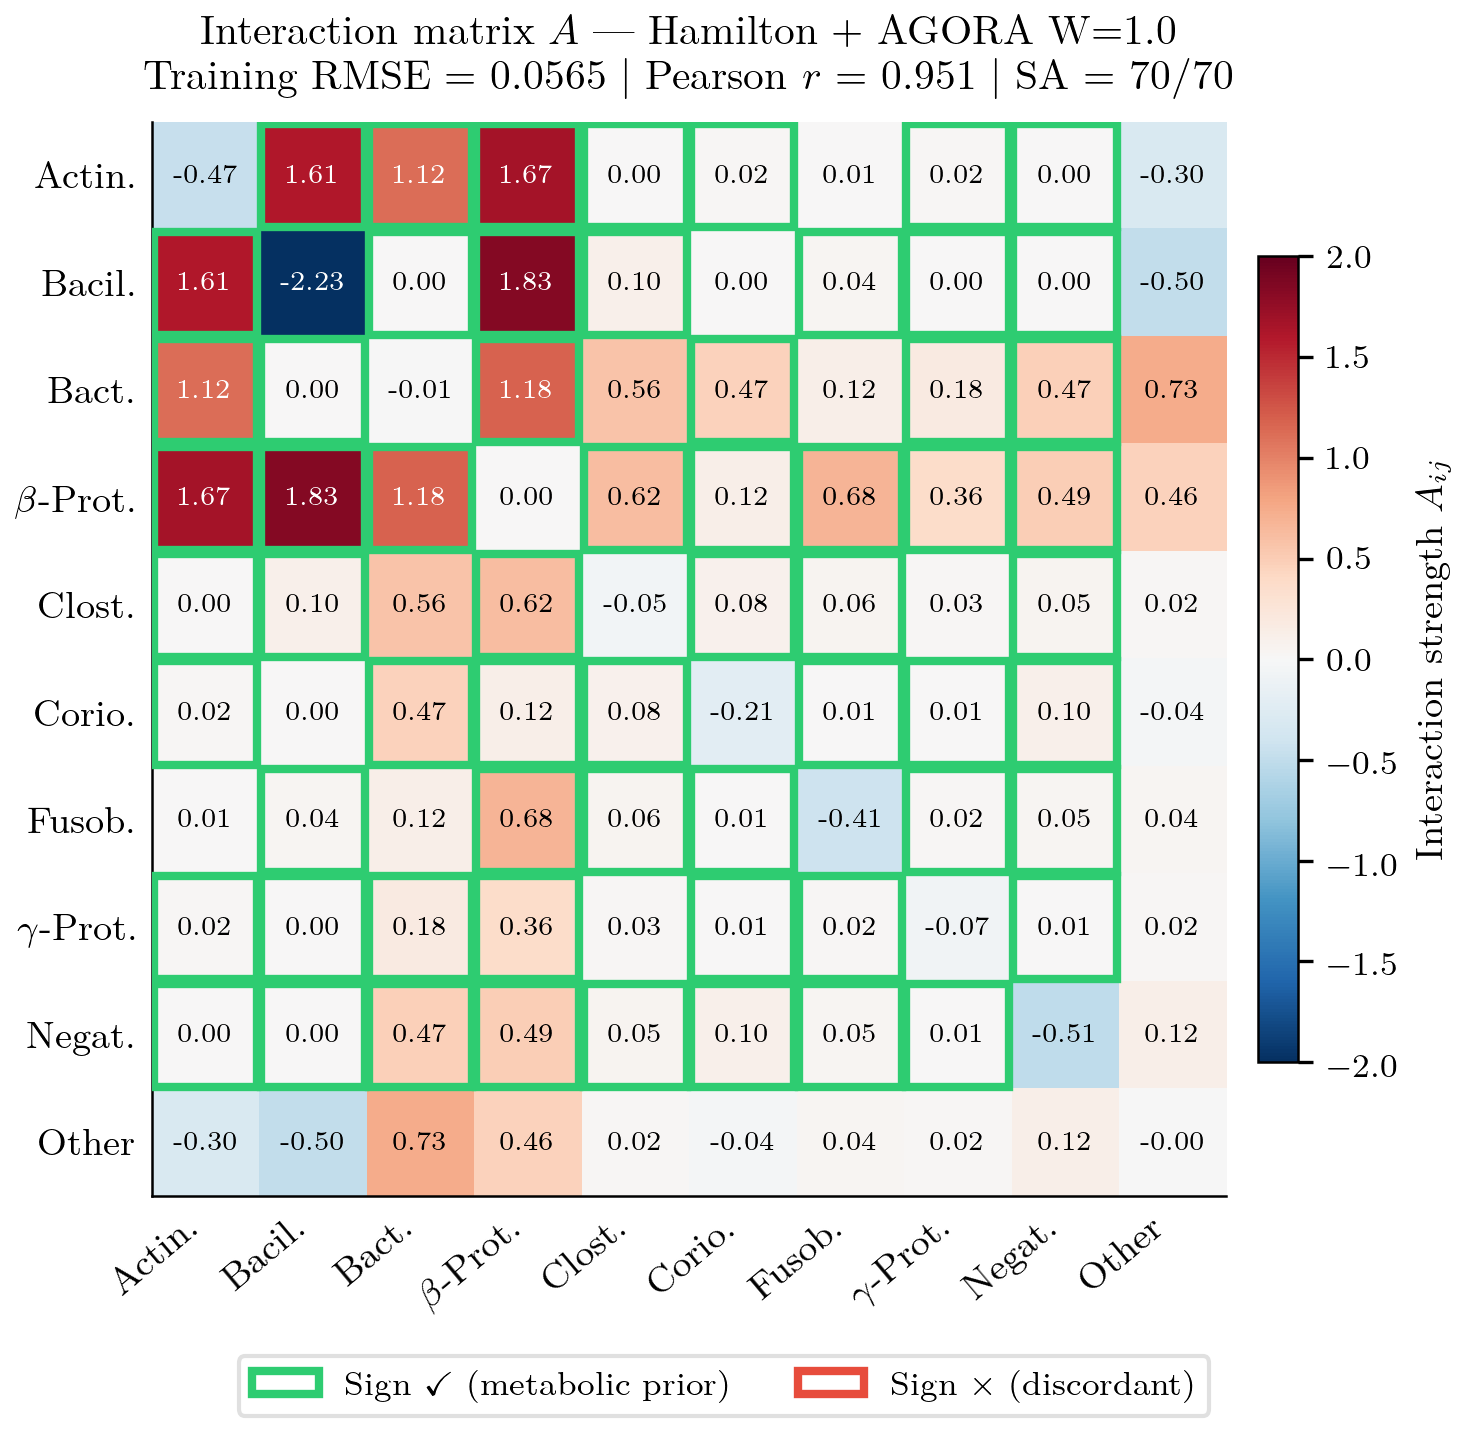
\includegraphics[width=\linewidth]{figures/fig1_A_matrix.png}
  \caption{フィットされた $\bA$（赤：促進、青：競争）。全対角 $A_{ii}<0$。チェックマーク：符号一致 70/70。}
\end{subfigure}
\hfill
\begin{subfigure}[b]{0.48\textwidth}
  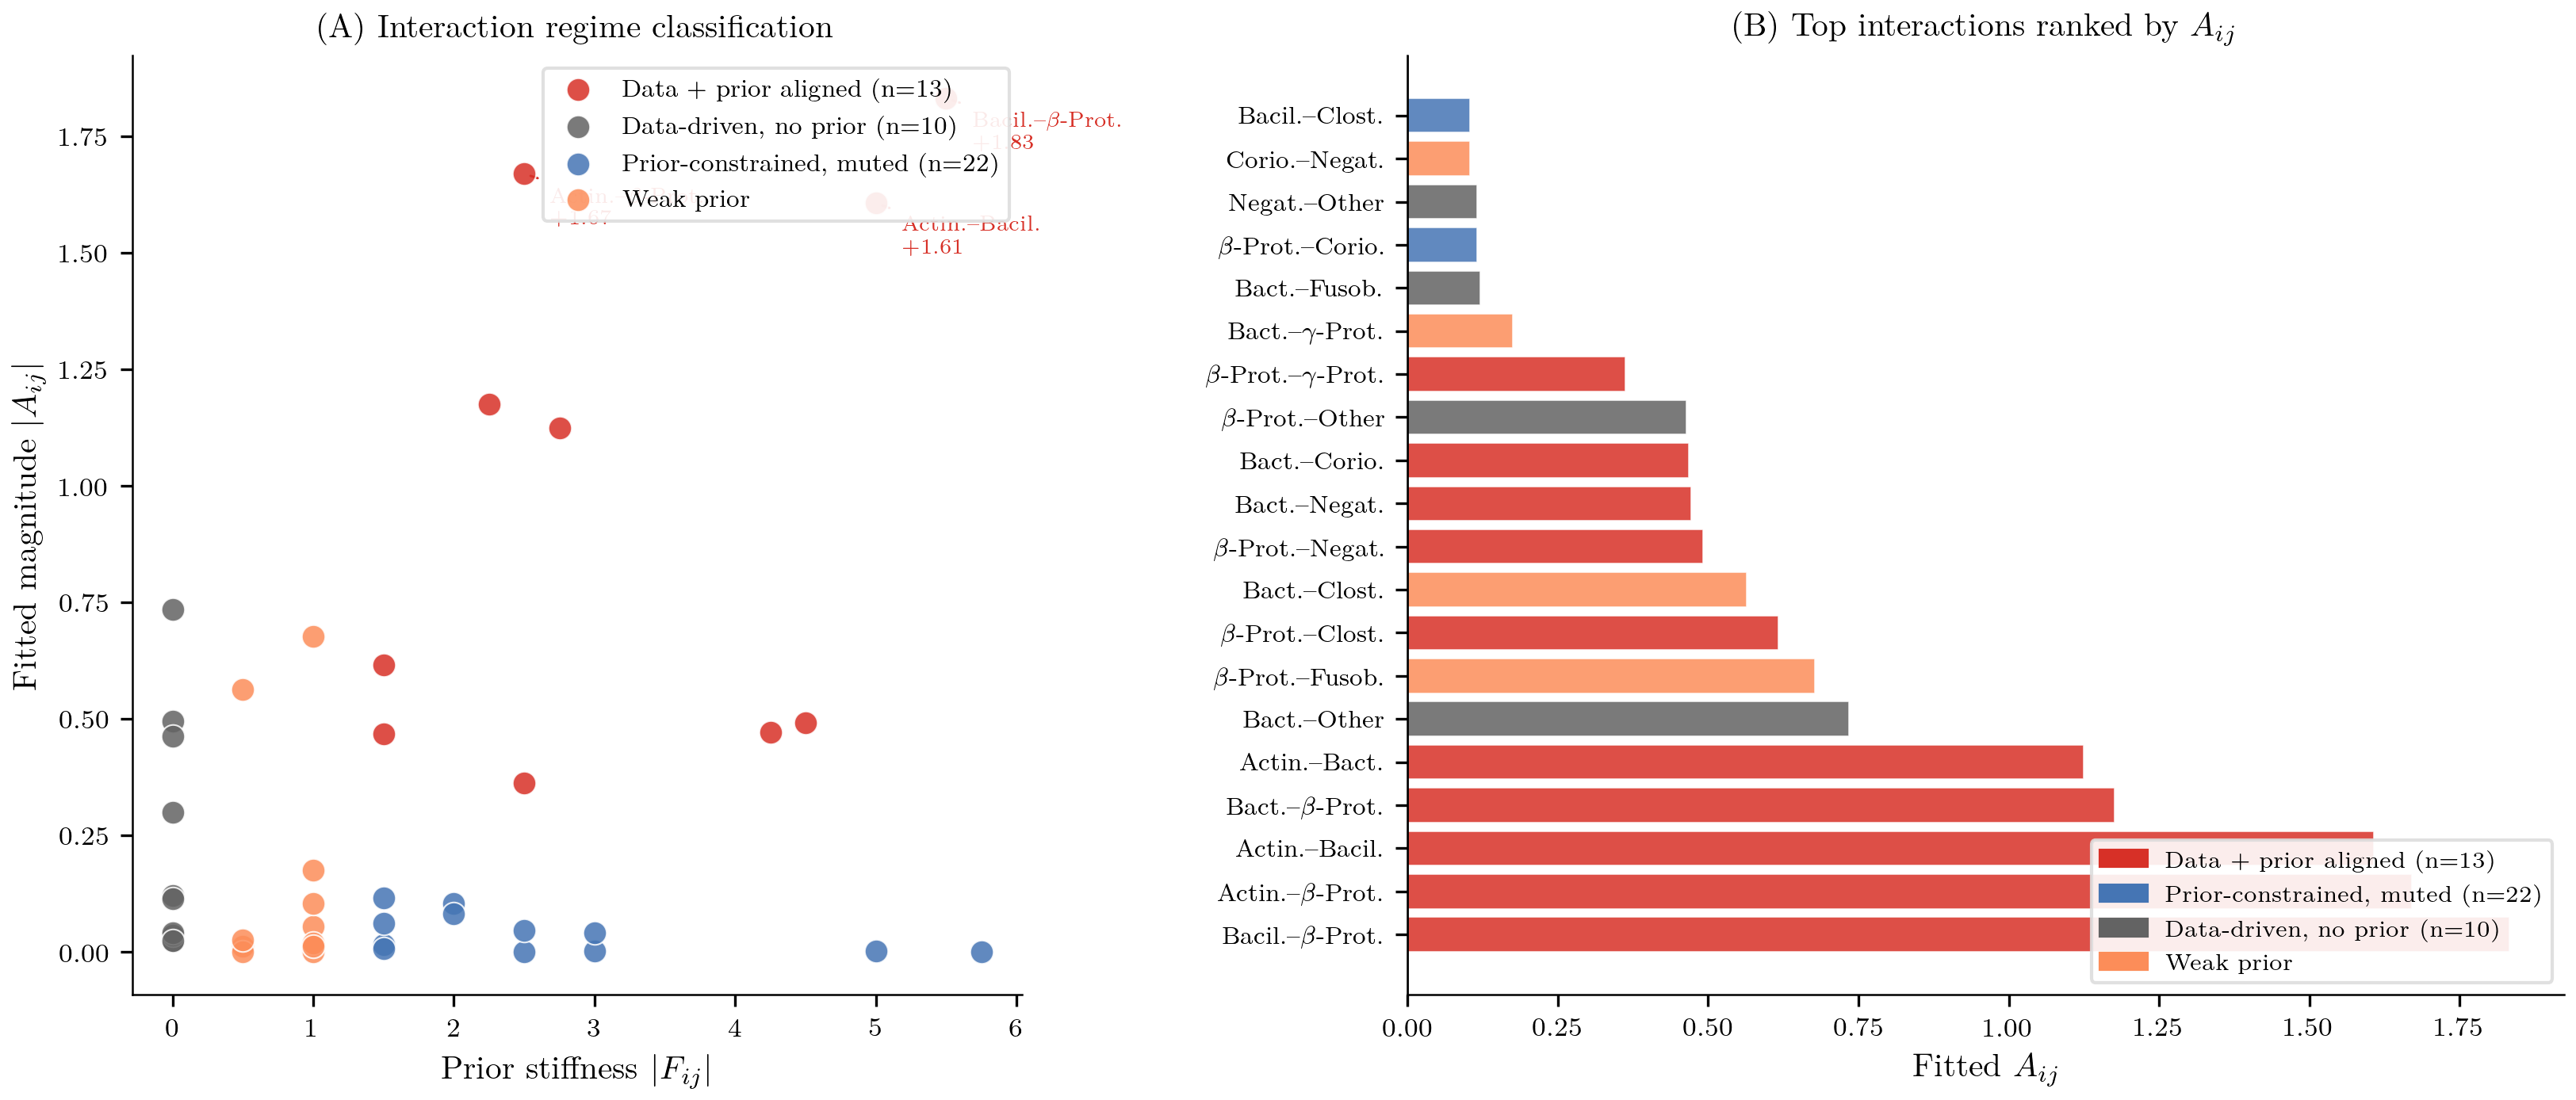
\includegraphics[width=\linewidth]{figures/fig5_A_biological.png}
  \caption{生態学的レジーム分類（プライア剛性 vs フィット大きさ）。}
\end{subfigure}
\caption{学習された相互作用行列と 3 つの生態学的レジーム。}
\end{figure}

45 の非対角ペアは以下の 3 レジームに分類される：
\begin{description}[noitemsep]
  \item[データ+プライア整合（13 ペア）：] $|A_{ij}|>0.3$ かつ $|F_{ij}|>1$。
        全 10 LOO フォールドで符号一致率 SC$=1.00$。
        代表例：Actinobacteria--Bacilli（$A=+1.61$）、
        Bacilli--Betaproteobacteria（$A=+1.83$）、文献の共凝集共生と整合。
  \item[プライア拘束・弱（22 ペア）：] $|A_{ij}|<0.01$、$|F_{ij}|>1$。
        強い代謝的証拠があるが、3 週間スケールでは生態学的に弱い。
        代表例：Bacilli--Negativicutes（$A=+0.003$、乳酸菌--Veillonella 軸）。
  \item[データ主導・プライアなし（10 ペア）：] $|F_{ij}|=0$、$|A_{ij}|>0.05$。
        代謝アノテーションなし。主に ``Other'' ギルド周辺。
\end{description}

\subsection{コミュニティ構造と患者クラスタリング}

LOO 予測 vs 観測の W2/W3 組成に対する PCA/LDA 解析：
\begin{itemize}[noitemsep]
  \item 予測組成が観測と同じデータ多様体上に分布（平均回帰の失敗なし）。
  \item LDA による CT1/CT2 識別：LOO 条件下で \textbf{90\%}（患者 A のみ誤分類）。
  \item $\hat\bb^{(p)}$ の PCA：\textbf{ラベルなし}で PC1 が CT1 vs CT2 を分離。
  \item $|\bar A_\text{off-diag}|=0.35 > |\bar b|=0.18$：コミュニティ生態学が個人の成長率に優先。
\end{itemize}

\begin{figure}[H]
\centering
\begin{subfigure}[b]{0.48\textwidth}
  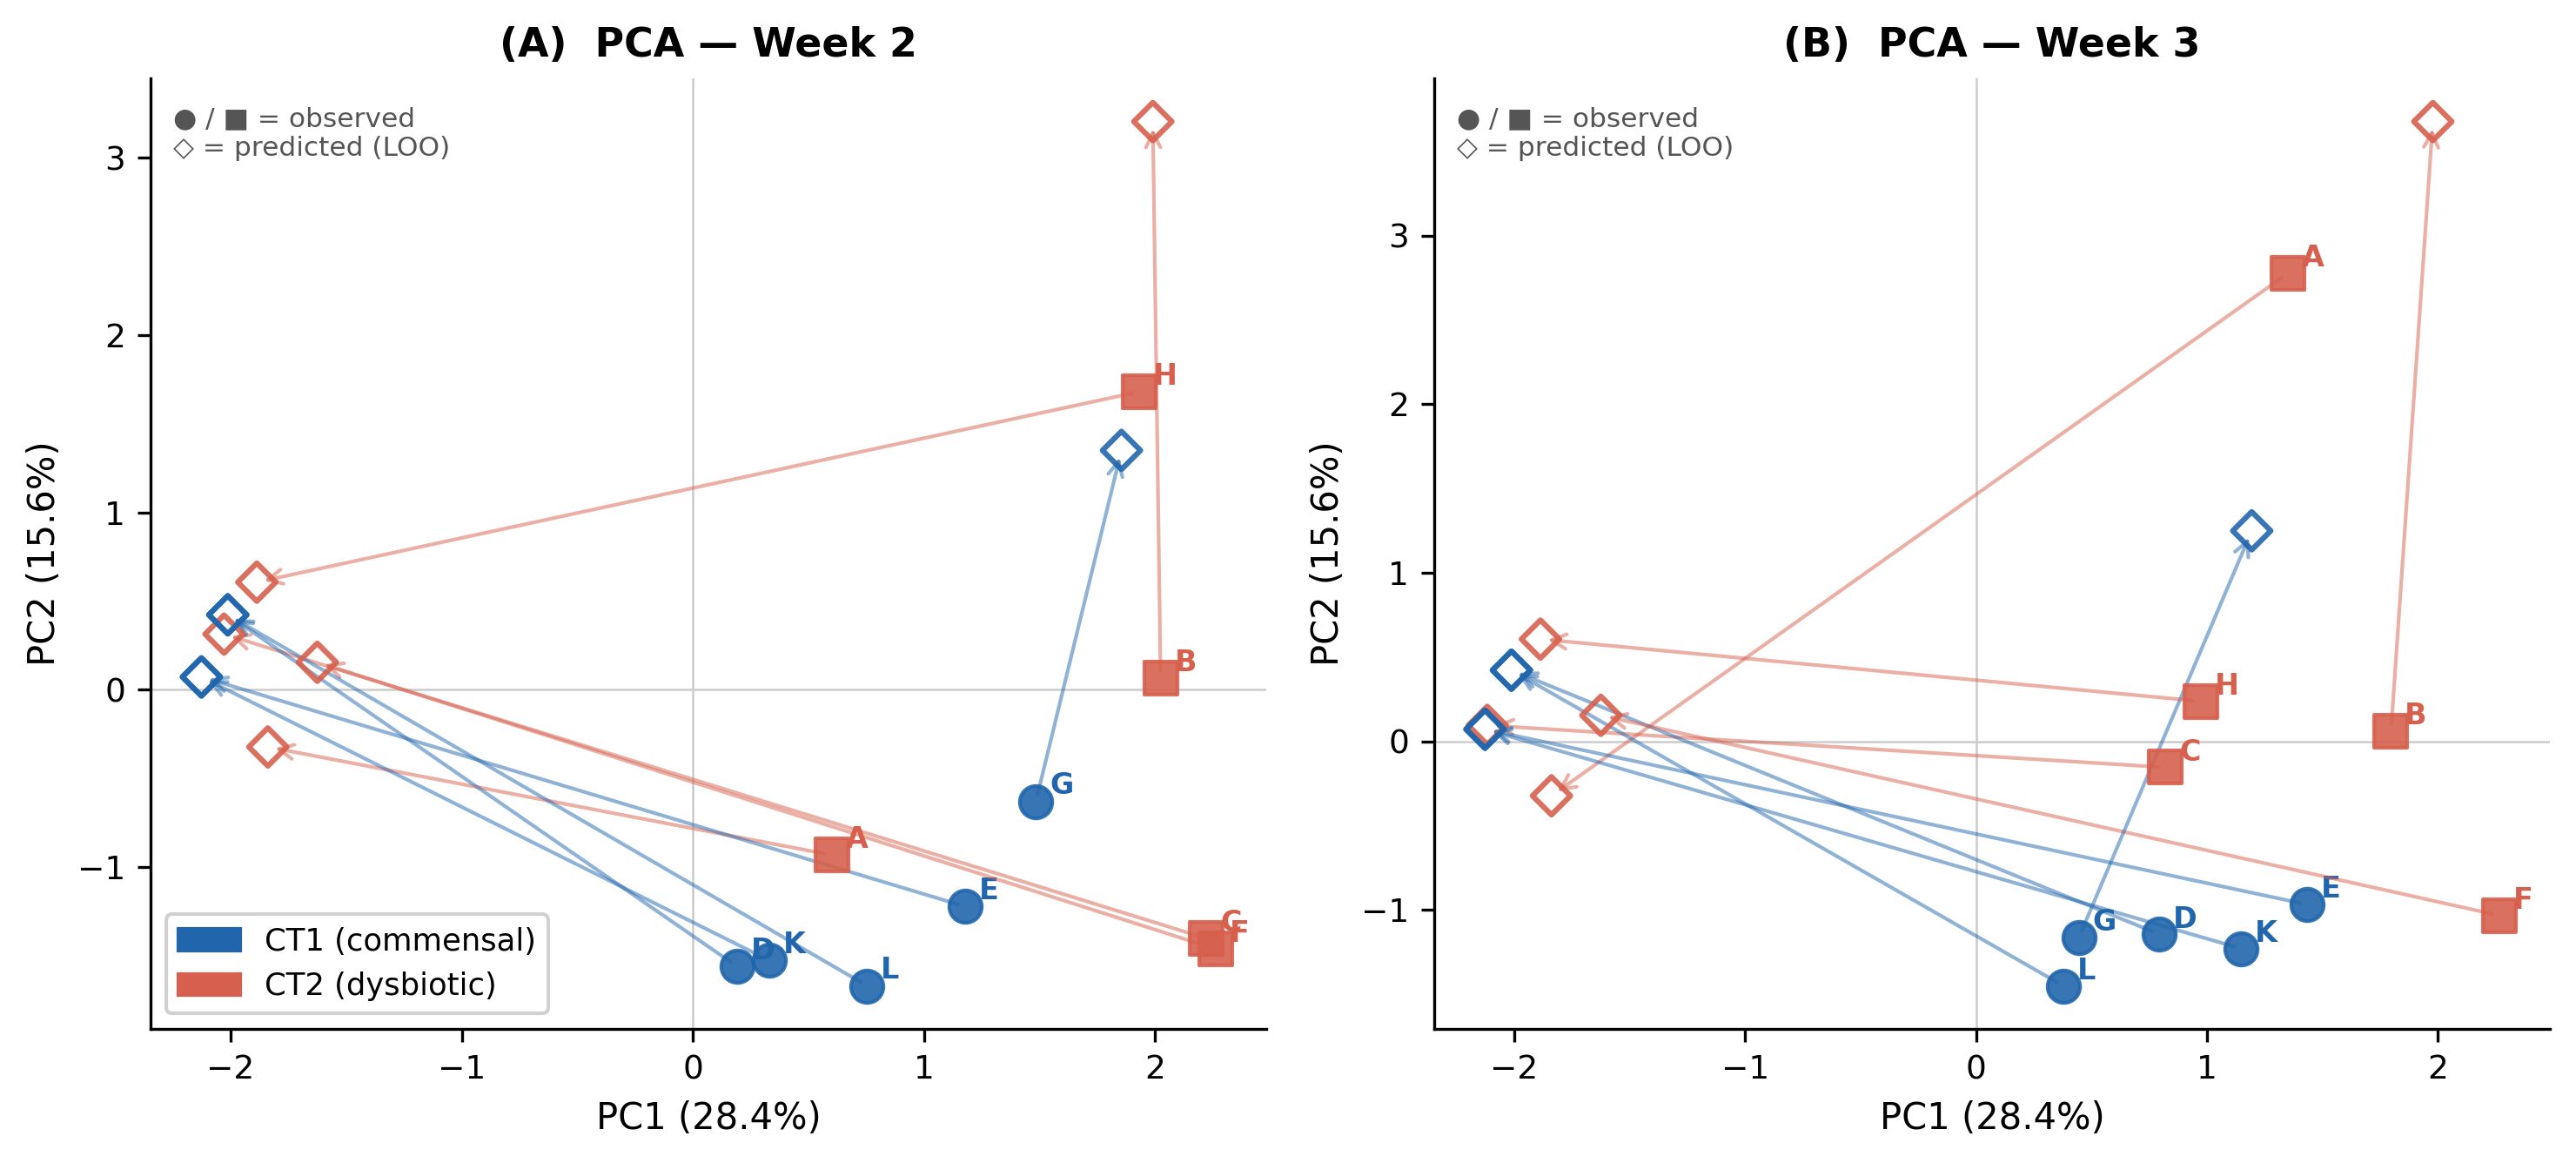
\includegraphics[width=\linewidth]{figures/fig_pca_pred_obs.png}
  \caption{PCA：予測（白抜き）が観測（塗り）を正しく追跡。}
\end{subfigure}
\hfill
\begin{subfigure}[b]{0.48\textwidth}
  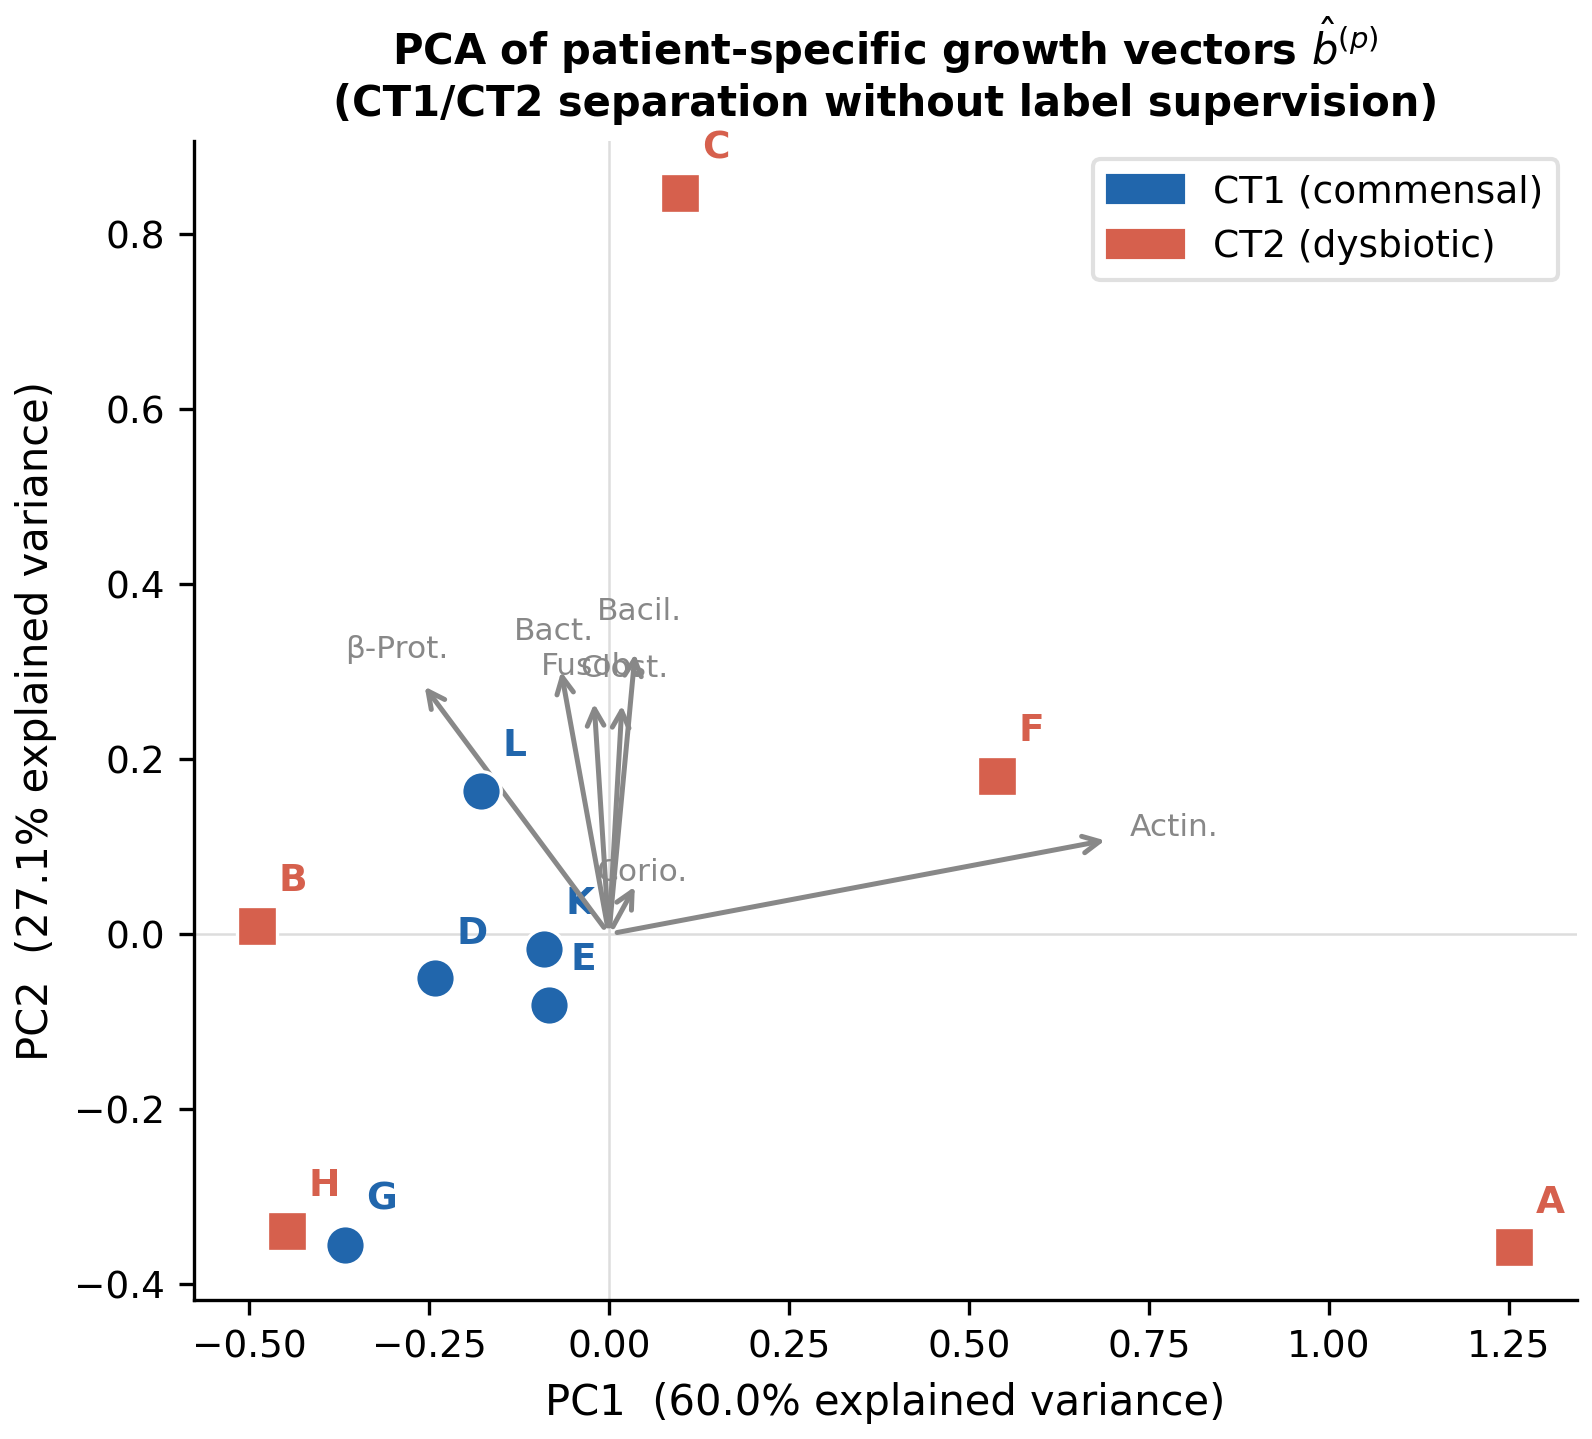
\includegraphics[width=\linewidth]{figures/fig4_b_pca.png}
  \caption{成長ベクトル $\hat\bb^{(p)}$ の PCA：ラベルなしで CT1/CT2 分離。}
\end{subfigure}
\caption{LOO 予測下のコミュニティ構造。}
\end{figure}

\subsection{AGORA 重みの相転移}

\begin{figure}[H]
\centering
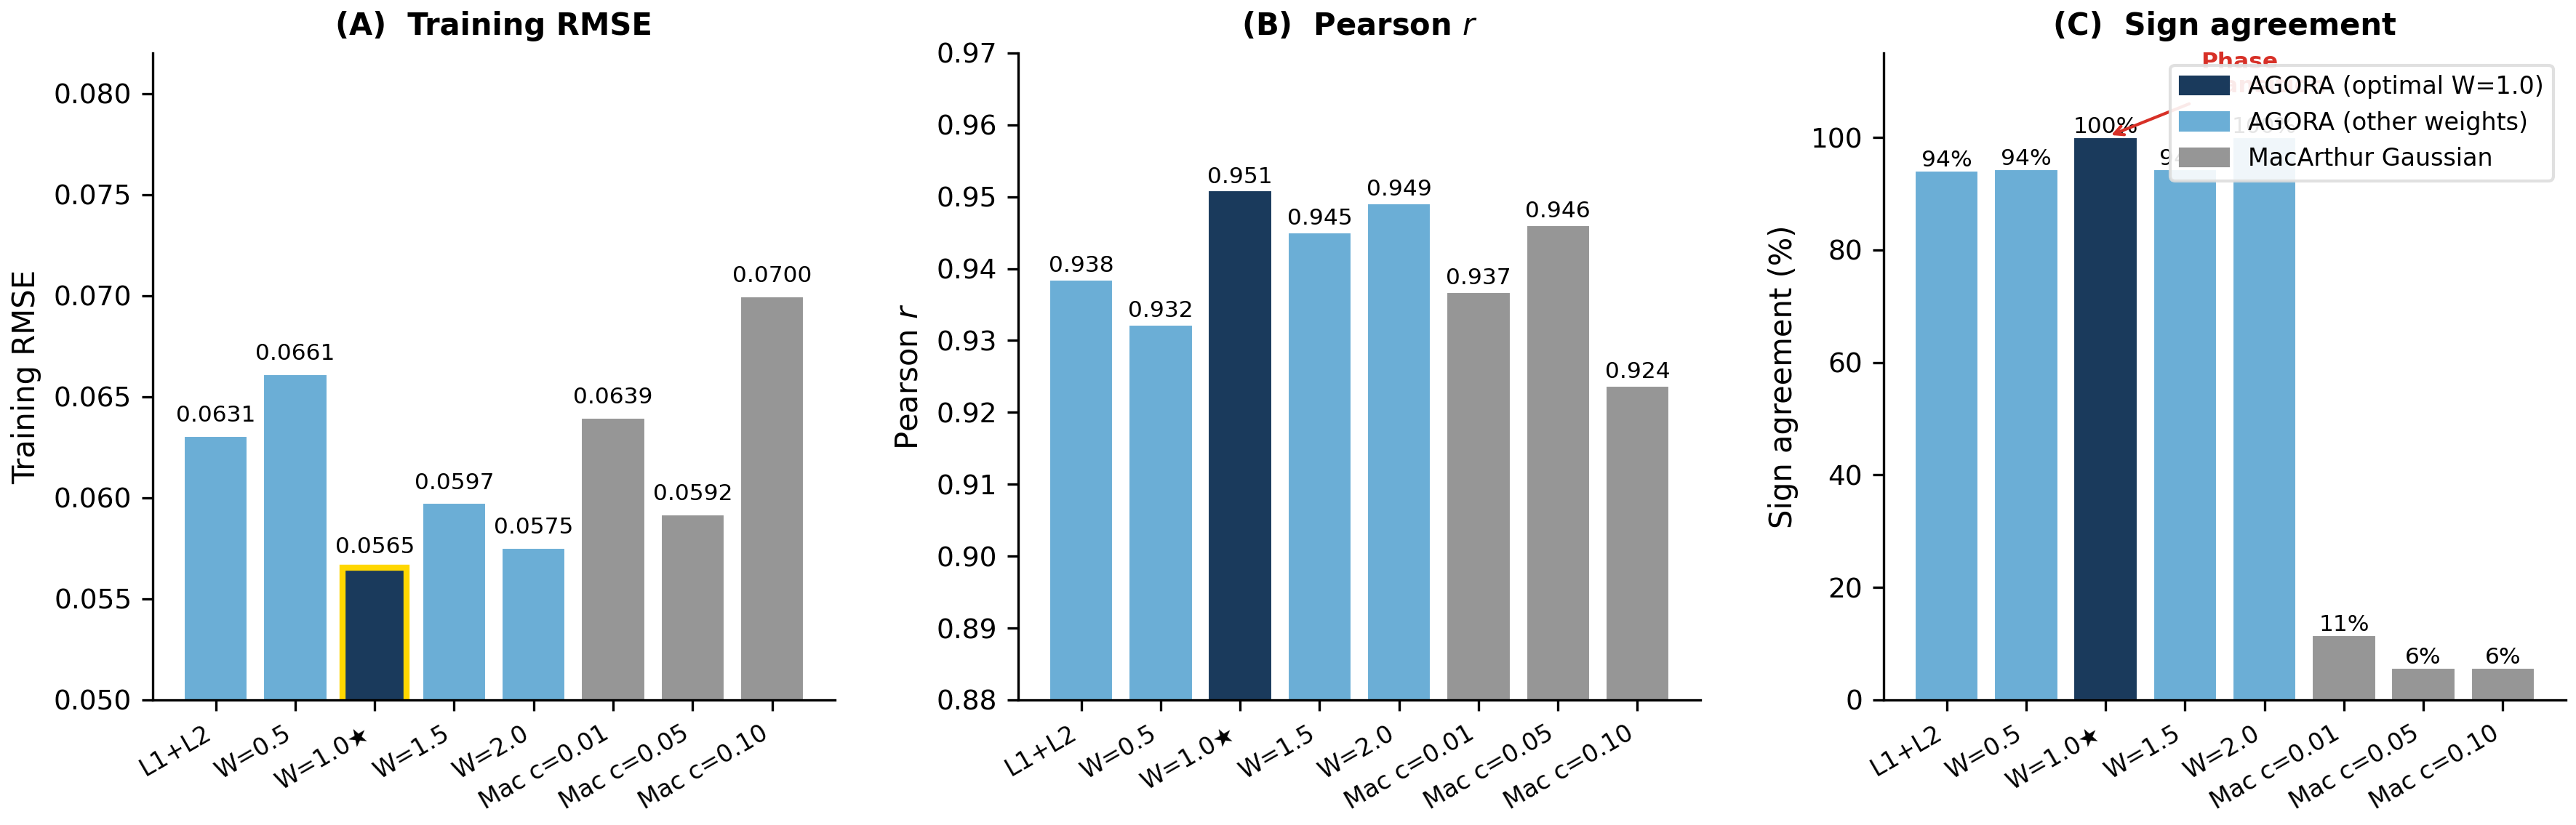
\includegraphics[width=0.88\linewidth]{figures/fig6_agora_weight_sweep.png}
\caption{AGORA 重みスイープ。$w=1.0$ で離散的相転移：SA が 94\% $\to$ 100\% に
ジャンプし同時に RMSE が最小化。MacArthur 型ガウスプライアは完全失敗（SA = 4--11/70）。}
\end{figure}

FBA は相互作用の\textbf{符号}は予測できるが、\textbf{大きさ}は予測できない。
単体上では $A_{ij}$ の符号のみが固定点を決定する（Hofbauer \& Sigmund 1998）。
この理論的予測を LOO-CV が実験的に裏付けた。

\subsection{外部検証：インプラント周囲炎の Dysbiosis}

\begin{figure}[H]
\centering
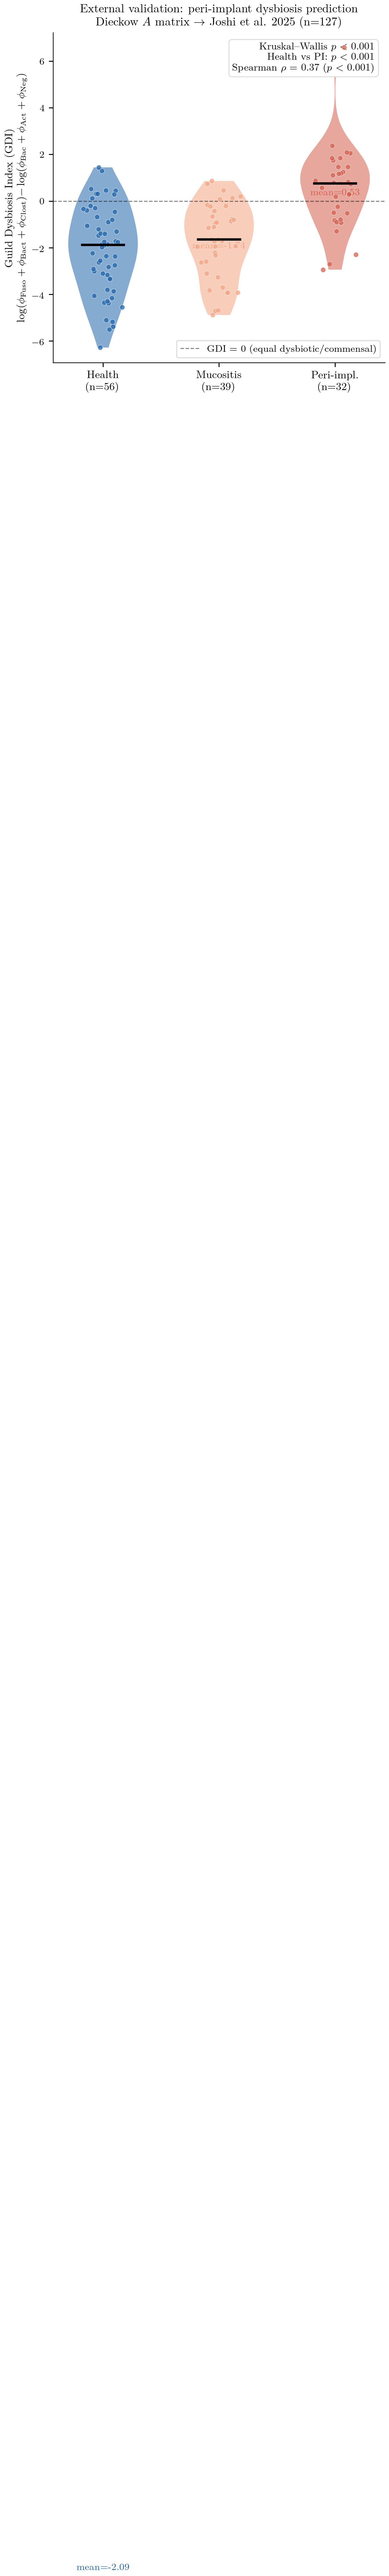
\includegraphics[width=0.70\linewidth]{figures/fig3_joshi_attractor.png}
\caption{Joshi et~al.~(2025) の 127 例インプラント周囲炎サンプルにおける
Guild Dysbiosis Index (GDI)。
健康・粘膜炎群は共生アトラクタ（GDI $\approx -3$）付近、
インプラント周囲炎群は Dysbiotic アトラクタ（GDI $\approx 0$）側へ有意偏位。}
\end{figure}

\begin{table}[H]
\centering\small
\caption{診断群別 Guild Dysbiosis Index（Joshi 2025、$N=127$）。}
\begin{tabular}{lcccc}
\toprule
診断 & $n$ & 平均 GDI & 中央値 GDI & vs 健康 \\
\midrule
健康                   & 56 & $-2.90$ & $-3.69$ & --- \\
粘膜炎                 & 39 & $-3.05$ & $-3.67$ & $p=0.61$ \\
インプラント周囲炎      & 32 & $-0.29$ & $+0.48$ & $p<0.0001$ \\
\bottomrule
\multicolumn{5}{l}{\small Kruskal-Wallis $H=30.4$、$p<0.0001$。Spearman $\rho=0.37$、$p<0.0001$。}
\end{tabular}
\end{table}

10 患者・3 週間のう蝕回復データから推定した $\bA$ が、
全く独立した 127 例のインプラント周囲炎横断データで
重症度を正しく順序付けた。
アトラクタ構造が $\bA$ のみで決定されるという理論予測の実験的支持。

% ── 4. 限界と今後の課題 ──────────────────────────────────────────────
\section{限界と今後の課題}

\begin{limitbox}[限界]
\begin{enumerate}[noitemsep]
  \item \textbf{サンプル数不足。} $N=10$、$p=0.08$（$\alpha=0.05$ で非有意）。統計的検出力確保には $N \geq 30$ が必要。
  \item \textbf{対称制約。} $A_{ij}=A_{ji}$ は片利共生・片害共生を除外。大規模コホートでは非対称モデルが有利になる可能性。
  \item \textbf{ギルド集約の粗さ。} クラスレベルでは菌種間相互作用が相殺・強化される可能性。
  \item \textbf{プライア文脈不一致。} L1 はう蝕文脈の eHOMD に基づく。歯周炎データ（Duran-Pinedo 2021）では効果 $< 0.1\%$ RMSE（不一致を示唆）。
  \item \textbf{単一時点 $b$ 推定。} LOO の $\hat b^{(p)}$ は W1 のみから推定；主に $\bA$ の汎化を検証。
  \item \textbf{Joshi マッピング近似。} 10 ギルド中 5 つを Dieckow 平均で補完；定常性（平衡近傍）未検証。
\end{enumerate}
\end{limitbox}

\textbf{今後の方向性：}
(1) $N \geq 30$ での再現実験；
(2) 非対称 gLV + 非対称サインプライア；
(3) 歯周炎特異的プライア構築；
(4) TMCMC によるベイズ不確かさ定量化（Nishioka et~al., 準備中）；
(5) 菌株近似を超えるコミュニティ FBA（MICOM）の導入。

% ── 5. 結論 ──────────────────────────────────────────────────────────
\section{結論}

\begin{keybox}[まとめ]
eHOMD 実験フロー + AGORA2 pFBA による 3 層代謝サインプライアと
Hamilton Replicator 力学の組み合わせは、経口マイクロバイオーム組成予測で真の汎化性能を達成した：
\begin{itemize}[noitemsep]
  \item \textbf{符号一致率 100\%}（70/70 拘束ペア、AGORA W$=1.0$）
  \item \textbf{LOO-RMSE $-14\%$}（非拘束 gLV 比：0.0504 vs 0.0588）
  \item \textbf{LOO-BC $-48\%$}（持続性ヌル比：0.147 vs 0.281）
  \item \textbf{CT識別精度 90\%}（LOO 条件下、ラベルなし $\hat b$ クラスタリング）
  \item \textbf{外部検証：} Dieckow $\bA$ が 127 例独立データで Dysbiosis を正しく順序付け（$p<0.0001$）
\end{itemize}
FBA の符号情報は代表菌株近似・培地近似の誤差に対して頑健に生き残る。
サインプライアは符号が曖昧なパラメータ方向を除去することで汎化を妨げる過適合を防ぐ
ハーフスペース正則化として機能する。
定量的改善は $p=0.08$（$N=10$ のため限定的）だが、
生物学的整合性（7/10 名、正しい指標順序、構造的 PCA/LDA 妥当性）が真の予測的価値を支持する。
\end{keybox}

\bigskip
\noindent\small\textbf{主要参考文献：}
Dieckow et~al.~(2024) \textit{npj Biofilms Microbiomes} 10:85 $\cdot$
Joshi et~al.~(2025) \textit{npj Biofilms Microbiomes} 11:175 $\cdot$
Heinken et~al.~(2023) \textit{Nature Biotechnology} 41:1320 $\cdot$
Klempt et~al.~(2024) \textit{Biomechanics Modeling Mechanobiol.} 23 $\cdot$
Hofbauer \& Sigmund (1998) Cambridge UP $\cdot$
Szafra\'{n}ski et~al.~(2025) [preprint].

\end{document}
